%!TEX root = ../../book_ML.tex
\chapter{Triển khai chương trình và đánh giá hiệu suất}
\label{cha:chap3}
% \index{principal component analysis}
% \index{PCA -- \textit{xem} principle component analysis}
% \index{PCA}

% \index{phân tích thành phần chính -- principle component analysis}
% \index{principle component analysis -- phân tích thành phần chính}
% \index{PCA}
\section{Triển khai chương trình}
Về cơ bản để triển khai một bộ mã hóa tự động cho bài toán nén 
có các bước chính sau:
\begin{itemize}[leftmargin=1.5cm]
    \item Thiết kế các lớp mạng
    \item Lựa chọn hàm đánh giá mất mát
    \item Lựa chọn thuật toán tối ưu
    \item Huấn luyện mô hình với tập dữ liệu cần nén
    \item Thực hiện nén, giải nén
\end{itemize}

Hoạt động nén được chia thành 2 quy trình:
\begin{itemize}[leftmargin=1.5cm]
    \item Huấn luyện mô hình (đại diện thao tác nén)
    \item Thực hiện nén, giải nén tập dữ liệu đã huấn luyện
\end{itemize}

\subsection{Thiết kế các lớp mạng}
\subsection{Lựa chọn hám đánh giá mất mát}
\subsection{Lựa chọn thuật toán tối ưu}
\subsection{Huấn luyện mô hình với tập dữ liệu cần nén}
\subsubsection{Tập dữ liệu sử dụng}

Ở đây, để tăng tính ngẫu nhiên chúng em sử dụng 1 tập dữ liệu ảnh màu với các 
kích thước giống nhau (768x1280) được cung cấp từ một thư viện lấy các ảnh ngẫu 
nhiên từ các video trên nền tảng Youtube. Với số lượng là 2286 ảnh chất 
lượng cao, tổng dung lượng lưa trữ là 6.3 GB

\begin{figure}
    \begin{subfigure}{0.6\textwidth}
        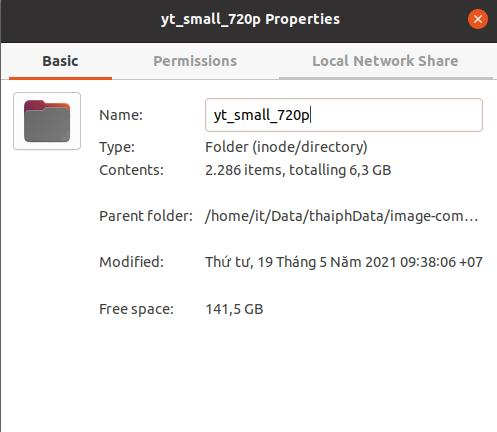
\includegraphics[width=1.\linewidth]{Chapters/items/data.jpg}
        \caption{}
        \label{fig: data}
    \end{subfigure}
    \caption{Tập dữ liệu sử dụng}
\end{figure}

\subsubsection{Các tham số huấn luyện mô hình}
Khi huấn luyện một mô hình mạng nơ-ron nhận tạo điển hình có 
các tham số như là : số kỷ nguyên (epoch), Kích thước lô (batch size), 
số lân lặp lại (Iterations)

Đối với mô hình này chúng ta phải lựa chọn thêm 1 số tham số giống như 
số luồng (thread), tỷ lệ học (learning rate) để mô hình trở lên linh hoạt hơn

Với GPU Tesla T4 16GB, được cung cấp bởi Google Colab và dữ liệu 
2286 ảnh chúng em lựa chọn các tham số kích thước lô là 16, số kỷ nguyên là 3,
tỉ lệ học tập là 0,0001, số luồng chạy là 5

\begin{figure}
    \begin{subfigure}{0.7\textwidth}
        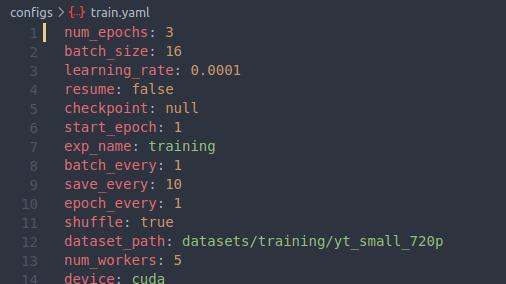
\includegraphics[width=1.\linewidth]{Chapters/items/pram.jpg}
        \caption{}
        \label{fig: param}
    \end{subfigure}
    \caption{Các tham số được lựa chọn}
\end{figure}

\subsubsection{Quá trình huấn luyện mô hình}

Tổng thời gian khi huấn luyện mô hình là khoảng 30 phút, điều này 
đại diện cho thời gian nén mặc dù vẫn chưa thực sự tối ưu về mặt 
thời gian, nhưng chúng em tin rằng khi phần cứng mạnh mẽ hơn thì
thời gian nén cũng sẽ giảm đi đáng kể.

\begin{figure}
    \begin{subfigure}{0.8\textwidth}
        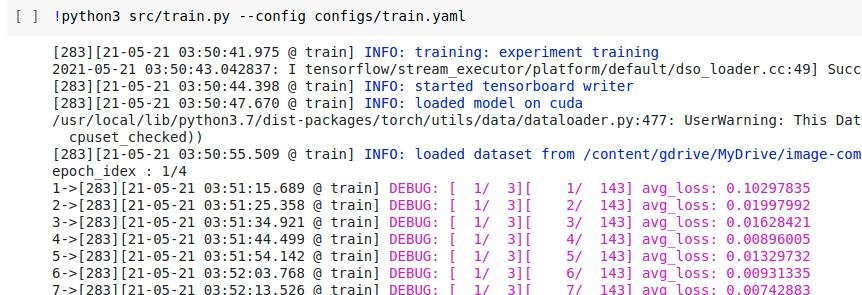
\includegraphics[width=1.\linewidth]{Chapters/items/colab1.jpg}
        \caption{}
        \label{fig: colab1}
    \end{subfigure}
    \caption{Khởi đầu quá trình huấn luyện}
\end{figure}

\newpage
Có thể thấy rằng tham số avg-loss (đánh giá sứ mất mát) từ lúc 
bắt đầu huấn luyện cho đến khi kết thúc đã giảm đi rất đáng kể
cho thấy tính đúng đắn của mô hình, dự báo rằng mô hình sẽ đạt kết
quả thử nghiệm tốt.

\begin{figure}
    \begin{subfigure}{0.8\textwidth}
        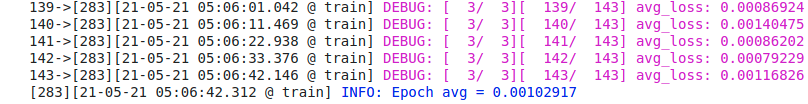
\includegraphics[width=1.\linewidth]{Chapters/items/colab2.jpg}
        \caption{}
        \label{fig: colab2}
    \end{subfigure}
    \caption{Kết thúc quá trình huấn luyện}
\end{figure}

Mô hình hóa quá trình huấn luyện sử dụng tensorboard :
(Trục ngang là số lần lặp lại, trục đứng là đánh giá mất mát)

\begin{figure}
    \begin{subfigure}{0.8\textwidth}
        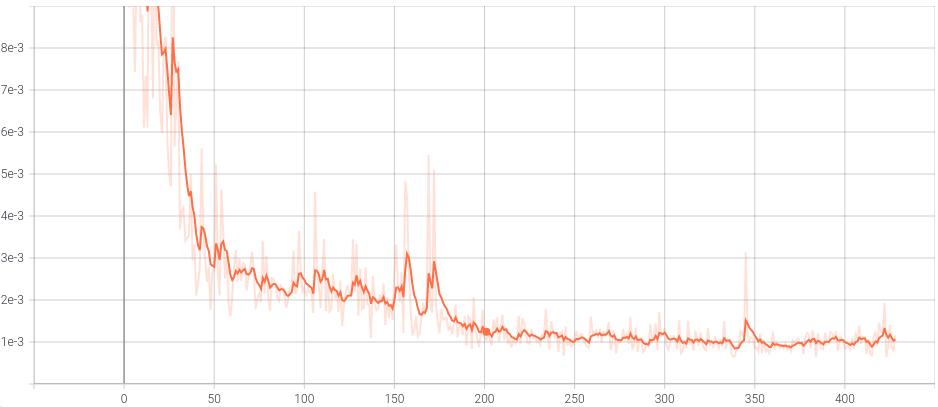
\includegraphics[width=1.\linewidth]{Chapters/items/visualizeTraining.jpg}
        \caption{}
        \label{fig: visualize}
    \end{subfigure}
    \caption{Quá trình giảm của mất mát theo số lần lặp lại các lô}
\end{figure}

\subsection{Thực hiện nén, giải nén}
\section{Đánh giá hiệu suất nén}


